%% eval.tex
%% $Id: eval.tex 61 2012-05-03 13:58:03Z bless $

\chapter{Evaluation}
\label{ch:Evaluierung}
%% ==============================

Die Implementierung nichtlinearer Taylormodelle ergibt eine Vielzahl von Konfigurationsmöglichkeiten und damit einen großen Suchraum nach der optimalen Einstellung:
\begin{itemize}
 \item Grenzwert für Cleaning $\delta_c$, Splitting $\delta_s$
 \item Grad der Reduktion durch Sweeping
 \item Anzahl der zu erhaltenden Fehlersymbole
 \item Strategie beim Sweeping
 \item Heuristik für die Reihenfolge, in der Fehlersymbole gesweept werden
 \item Vorgehen beim Splitting
 \item Definition des initialen Taylormodells
\end{itemize}
Diese Konfigurationen werden in \verb+hotm+ als JSON-Datei mit Hilfe einer JSON-Bibliothek\footnote{\url{https://github.com/nlohmann/json} (Stand Dezember 2020)} eingelesen und verarbeitet, um wiederholte Durchläufe mit leicht veränderten Parametern oder Batch-Runs zu vereinfachen. Listing \ref{list:config} zeigt ein Beispiel einer Konfigurationsdatei, mit der versuchsweise 1000 Iterationen der H\e non-Abbildung berechnet werden sollen. 



\section{Housekeeping-Grenzwerte}
Der Grenzwert einer Housekeeping-Methode gibt an ab welchem Wert die jeweiligen Methoden angewandt werden. Bei einem intervall in \verb+hotm+ $[m \pm r]$ mit $m = [c_m \pm \varepsilon_m]$ und $r = [c_r \pm \varepsilon_r]$ als \verb+iRRAM-REAL+s wird
\begin{itemize}
 \item Cleaning angewandt, wenn $\varepsilon_m < \delta_c$ oder $\varepsilon_r < \delta_c$ gilt und
 \item Splitting angewandt, wenn $c_m < \delta_s$ oder $c_m < \delta_s$ gilt.
\end{itemize}
Um diese Werte zu untersuchen, wurde betrachtet, wie sich die Größe des Rechtecks, welches durch die Intervalle $x$ und $y$ aufgespannt wird, abhängig von den Grenzwerten $\delta_c$ und $\delta_s$ auswirkt, beziehungsweise, wieviele Iterationen der H\e non-Abbildung bei einer festen Genauigkeit der \verb+iRRAM-REAL+s möglich sind, bis das Rechteck eine Fläche\footnote{Ab einer Fläche von zirka $2^-{5}$ ist die Überschätzung der Intervalle zu groß und wächst innerhalb weniger Iterationen ($< 10$) gegen $\infty$.} von $>2^{-5}$ erreicht hat.


\begin{table}[tbh]
\centering
\begin{tabular}{ll}
\begin{tabular}{|l|l||c|c|}
\hline \multicolumn{3}{|c|}{\begin{tabular}[c]{@{}c@{}}1000 Bits Präzision \\$x=[0 \pm 2^{-1000}], y=[0 \pm 2^{-1000}]$\\ \end{tabular}}                                                                                                                                                                                                                              \\ \hline
\multicolumn{1}{|c|}{\begin{tabular}[c]{@{}c@{}}$\delta_c$\\($2^{-\delta_c}$)\end{tabular}} & \multicolumn{1}{c||}{\begin{tabular}[c]{@{}c@{}}$\delta_s $\\($2^{-\delta_s}$)\end{tabular}} & \begin{tabular}[c|]{@{}c@{}}Iterationen \end{tabular}   \\ 
\hline
- & - & 451  \\
10   & 10       & 162     \\
10   & 5       & 160      \\
100  & 100      & 273     \\
100  & 50      & 258      \\
500  & 500      & 794     \\
500  & 250      & 746      \\
1000 & 1000     &  1432 \\                                   
1000 & 500    & 1317 \\                                    

\hline 
\end{tabular}
&
\begin{tabular}{|l|l||c|c|}
\hline \multicolumn{3}{|c|}{\begin{tabular}[c]{@{}c@{}}10000 Bits Präzision \\$x=[0 \pm 2^{-10000}], y=[0 \pm 2^{-10000}]$\\ \end{tabular}}                                                                                                                                                                                                                              \\ \hline
\multicolumn{1}{|c|}{\begin{tabular}[c]{@{}c@{}}$\delta_c$\\($2^{-\delta_c}$)\end{tabular}} & \multicolumn{1}{c||}{\begin{tabular}[c]{@{}c@{}}$\delta_s $\\($2^{-\delta_s}$)\end{tabular}} & \begin{tabular}[c|]{@{}c@{}}Iterationen \end{tabular}   \\ 
\hline
- & - & 4360  \\
100  & 100      & 1463     \\
100  & 50      & 1450      \\
1000 & 1000     &  2641 \\                                   
1000 & 500    & 2530 \\           
5000  & 5000      & 7849     \\
5000  & 2500      & 7289      \\
10000 & 10000     &  14455 \\                                   
10000 & 5000    & 13401 \\                                    
\hline 
\end{tabular}

\end{tabular}
\caption[Experimentelle Ergebnisse zu Grenzwerten]{Berechnung der Fläche des Rechtecks mit verschiedenen Grenzwerten für Cleaning $\delta_c$ und Splitting $\delta_s$ und festgelegter Präzision.}
\label{tab:housekeeping}
\end{table}

Tabelle \ref{tab:housekeeping} zeigt experimentelle Ergebnisse für $x_0 = 0 + 1 \cdot \lambda_1 $ und $y_0 = 0 + 1 \cdot \lambda_2$ mit $\lambda_1, \lambda_2 \in [0 \pm \varepsilon]$. Sowohl für 1000, als auch für 10000 Bits Genauigkeit reagiert das Ergebnis sehr sensibel auf die Grenzwerte der Housekeeping-Methoden. Falsch gewählte Werte vergrößern sogar die entstandene Überschätzung, im Vergleich zuer Berechnung ohne Cleaning und Splitting, jeweils in Zeile 1 der Tabellen zu sehen. Werden die Grenzwerte durch die \verb+iRRAM+-Präzision bestimmt, so bleibt der Fehler am längsten klein und die höchste Iterationszahl ist möglich.

\Abbildungps{tbh}{.6}{img/housesteps.png}{fig:housesteps}{Experimentelle Ergebnisse zu Grenzwerten}{Iterationszahl der H\e non-Abbildung mit fester Genauigkeit von 1000 Bits.}

Wie in Abbildung \ref{fig:housesteps} zu sehen ist, hat eine Definition der Grenzwerte unter die zugrunde liegende Genauigkeit keinen Effekt mehr auf die Performanz der Berechnung, da sich die Iterationszahl nicht weiter erhöht.  

\newpage
\section{Sweeping}
 Für eine Sweeping-Konfiguration kommen drei einander beeinflussende Parameter in Betracht: die Sweeping-Strategie, die Gradreduktion und die Anzahl der zu erhaltenen Fehlersymbole. Der Housekeeping-Vorgang für ein Taylormodell inklusive Sweeping besteht wiederum aus vier Schritten:
 \begin{enumerate}
  \item \textbf{(Sweeping)} Reduktion des Taylormodells bis zum angegebenen Grad, je nach Strategie
  \item \textbf{(Sweeping überschüssiger Fehlersymbole)} Entfernen aller Fehlersymbole bis auf die $n$-größten (abhängig von deren Support-Space)
  \item \textbf{(Cleaning)} Verlagern der durch die Schritte 1 und 2 entstandenen Rechenfehler auf der Ebene der \verb+iRRAM-REAL+s auf die Radii der Intervalle
  \item \textbf{(Splitting)} Einführen neuer Fehlersymbole für Monome, deren Koeffizienten durch die Schritte 1-3 zu stark gewachsen sind.
 \end{enumerate}

 Abbildung \ref{fig:sweeping} zeigt die Performanz der Berechnung der H\e non-Abbildung, gemessen an der erreichten Iterationszahl mit statischer Präzision in verschiedenen Fällen. Wie zuvor ist die Berechnung beendet, sobald die Fläche des Rechtecks einen Schwellenwert überschreitet. Zu sehen ist, bei welcher Kombination von Parametern für Sweeping (Schritt 1) und Sweping überschüssiger Fehlersymbole (Schritt 2) die Überschätzung am langsamsten wächst und somit die meisten Iterationen errechnet werden können. Die Zeiteffizienz ist in diesem Falle kein Faktor. Es ist zu erkennen, dass sich die Graphen innerhalb derselben Sweeping-Strategie kaum unterscheiden. Eine Verzehnfachung des Exponenten in der Breite der Intervalle und der Bits für die Präzision verzehnfacht auch die erreichte Iterationszahl. Die besten Ergebnisse werden beim Beschränken auf \textbf{square\_only} (quadratisches Sweeping) für $n=3$ und Sweeping zum Grade 0; bei \textbf{square\_first} für $n=1$, $n=4$ und Sweeping zum Grade 3 erreicht. Insgesamt wird jedoch mit \textbf{square\_only} zum Grade 0, also einem Sweeping bis zu einem Taylormodell, dessen Monome Variablen mit höchstens Grad 1 haben, die höchste Iterationszahl erzielt:

$$ c \cdot \lambda_1^3 \lambda_2^2 \lambda_3^1 \lambda_4^3  \underset{square\_only}{\overset{sweep\ to\ 0}{\rightsquigarrow}} c' \cdot \lambda_1^1 \lambda_2^0 \lambda_3^1 \lambda_4^1$$



\begin{figure}[tbh]
\centering
\begin{subfigure}{.5\textwidth}
  \centering
  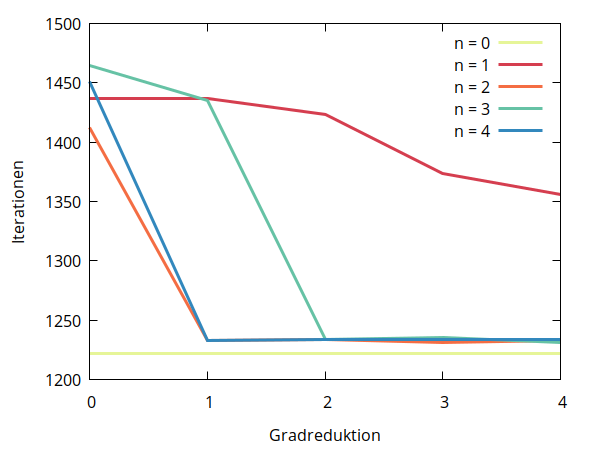
\includegraphics[width=\linewidth]{img/sweeping_only.png}  
  \caption{Sweeping beschränkt \textbf{square\_only}}
  \label{fig:sub1}
\end{subfigure}%
\begin{subfigure}{.5\textwidth}
  \centering
  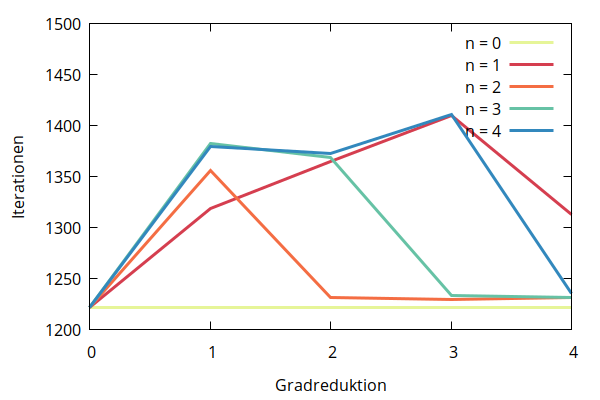
\includegraphics[width=\linewidth]{img/sweeping_first.png}
 \caption{Sweeping beschränkt \textbf{square\_first}}
  \label{fig:sub2}
\end{subfigure}

\begin{subfigure}{.5\textwidth}
  \centering
  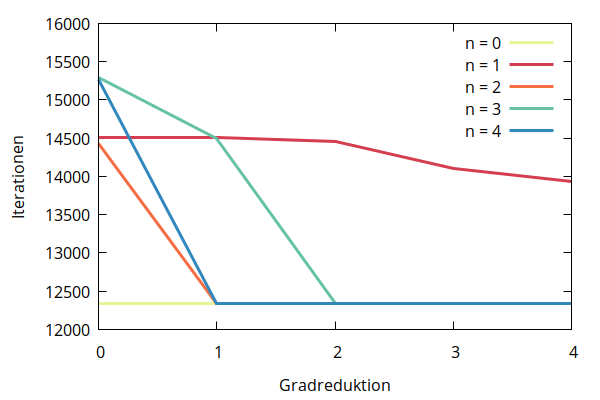
\includegraphics[width=\linewidth]{img/sweeping_only10k.png}
  \caption{Sweeping beschränkt \textbf{square\_only}}  
  \label{fig:sub1}
\end{subfigure}%
\begin{subfigure}{.5\textwidth}
  \centering
  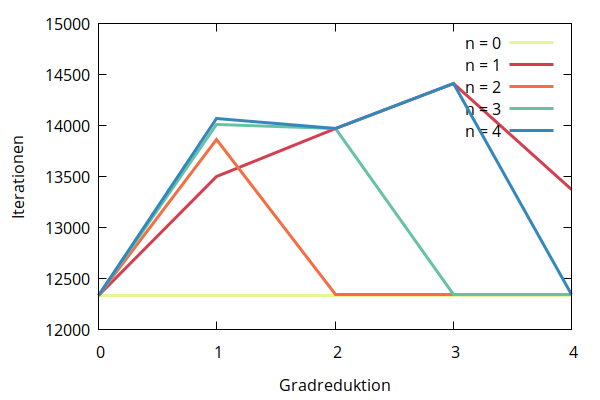
\includegraphics[width=\linewidth]{img/sweeping_first10k.png}
 \caption{Sweeping beschränkt \textbf{square\_first}}
  \label{fig:sub2}
\end{subfigure}
\caption[Sweeping mit verschiedenen Graden]{Anzahl an Iterationen mit Erhalt der n größten Fehlersymbole. (a) (b): 1000 Bits Präzision , $x_0 = y_0 = [0 \pm 2^{1000}]$.
 (c)(d): 10000 Bits Präzision , $x_0 = y_0 = [0 \pm 2^{10000}]$
}
\label{fig:sweeping}
\end{figure}

Im Vergleich mit rein linearen Taylormodellen zeigt sich eine Verbesserung (siehe Abbildung \ref{fig:extra}). Der Unterschied besteht darin, dass die nichtlinearen Taylormodelle während der Berechnung und besonders während der Multiplikation Punktintervalle erhalten können und sich stattdessen der Grad des Polynoms erhöht. Nach jeder Iteration werden diese dann zunächst im Grad reduziert, um diesen dann durch Splitting auf den Monomen um maximal 1 zu erhöhen. Für lineare Taylormodelle steht lediglich das Splitting für den Kernel zur Verfügung, da sonst nichtlineare Polynome entstünden. Des Weiteren wird hier bereits während der Multiplikation gesweept und Punktintervalle werden zu regulären Intervallen. Die Performanz des Sweepings \textbf{square\_only} zum Grade 0 verbessert sich im Schnitt mit einer wachsenden Zahl der zu erhaltenen Fehlersymbole, wie in Abbildung \ref{fig:extra} zu sehen ist. Jedes Fehlersymbol erhöht die Menge an erhaltener Abhängigkeitsinformation und sorgt dafür, dass ein Taylormodell dessen Ränder besser beschreiben kann. Allerdings stellt die Praktikabilität dieser Herangehensweise ein Problem dar, da so sehr große Polynome entstehen, die während einer Iteration der H\e non-Abbildung exponentiell in ihrer Länge wachsen. 
 

 \Abbildungps{tbh}{.7}{img/extra.png}{fig:extra}{Experimentelle Ergebnisse zu erhaltenen Fehlersymbolen}{Gegenüberstellung von $x_0 = y_0 = [0 \pm 2^{10000}]$ als lineare Taylormodelle und nichtlineare Taylormodelle mit quadratischem Sweeping zum Grade 0. Jeweils bleiben verschiedene Anzahlen von Fehlersymbolen pro Iteration erhalten. Gemessen wird die Iterationszahl der H\e non-Abbildung mit fester Genauigkeit von 10000 Bits, bis $|x_n|\cdot|y_n|$ einen Grenzwert von $2^{-6}$ überschreitet. }

 Dieser Effekt ist in Tabelle \ref{tab:time} zu sehen. Eine Erhöhung der Anzahl der erhaltenen Fehlersymbole hat einen drastischen Einfluss auf die Durchschnittliche Dauer einer Iteration in $ms$, bis das Programm bei größeren Werten quasi nicht mehr lauffähig ist ($>100ms$ pro Iteration). Betrachtet man nun das Verhältnis zwischen der Verbesserung der Performanz (Abbildung \ref{fig:extra}) und der Verschlechterung der Laufzeit (Tabelle \ref{tab:time}), so bildet das Setzen der erhaltenen Fehlersymbole auf 3 mit einem Zielgrade von 0 bei der Beschränkung auf quadratisches Sweeping einen guten Trade-off, weshalb diese Konfiguration als Voreinstellung für Sweeping in der Implementierung (Kapiter \ref{ch:umsetung}) vorgesehen ist.
 
  
 \begin{table}[tbh]
\centering
\begin{tabular}{|c||c|c|c|c|c|}
\hline
&\multicolumn{5}{c|}{Erhaltene Fehlersymbole pro Iteration} \\
\hline
Gradreduktion & 0 & 1 &2& 3 & 4\\
\hline
0& 0.166& 0.603&    2.097&   4.358&    13.354\\
1& 0.166& 0.939&   2.358&  7.470&   >100\\
2& 0.166& 1.645&     5.750&   20.339 &    >100\\
3& 0.166& 2.284&     2.977&   74.172&    >100\\
4&0.166& 2.658&    3.622&   >100    &   >100\\
\hline 
&\multicolumn{5}{c|}{$ms$ pro Iteration} \\
\hline
\end{tabular}

\caption[Experimentelle Ergebnisse zu erhaltenen Fehlersymbolen]{Durchschnittliche Dauer einer Iteration der H\e non-Abbildung in $ms$ mit Taylormodelle der Größe $[0\pm 2^{-10000}]$ bei festgelegter Präzision von 10000 Bits und 1000 Iterationen.}
\label{tab:time}
\end{table}
 
 
 \section{Cleaning}
 Durch die mehrstufige Intervallstruktur in den Koeffizienten der Polynome ist es mit Cleaning möglich, den Rechenfehler, beziehungsweise die Intervallbreite der Intervallgrenzen auf einer höheren Abstraktionsebene zu verwalten. Wie in Paragraph \ref{par:cleaning} beschrieben, wird das Intervall um die Intervallbreite des Mittelpunktes und des Radius' erweitert und schließt es somit komplett ein. Dies hat darüber hinaus den Effekt, dass sämtlicher entstandene Rechenfehler durch Splitting reduziert werden kann. 
 
   \Abbildungps{tbh}{.7}{img/clean.png}{fig:clean}{Experimentelle Ergebnisse zum Effekt des Cleaning}{Iterationszahl der H\e non-Abbildung mit festem Radius der intialen Taylormodelle $x_0 = y_0 = [0 \pm 2^{-1000}]$ mit wachsender Präzision, um den Effekt des Cleanings beschreiben.}
 
 Abbildung \ref{fig:clean} zeigt die Auswirkung der Anwendung von Cleaning bei initialen Taylormodellen $x_0, y_0$ der Breite $2^{-1000}$ mit wachsender Genauigkeit. Cleaning sorgt für ein langsameres Wachstum des Rechtecks $|x_n|\cdot|y_n|$ nach $n$ Iterationen im Vergleich zur Berechnung ohne Cleaning. Bei einer höheren Anzahl der erhaltenen Fehlersymbole pro Iteration wird der Effekt noch deutlicher, da nun mit deutlich längeren Polynomen gerechnet und dementsprechend mehr arithmetische Operationen auf den Koeffizienten angewandt werden. So bleibt zwar mehr Information über Form der Taylormodelle erhalten, jedoch dominiert die Überschätzung auf der Zahlenebene das Ergebnis beim Verzicht auf Cleaning, während sich die Performanz im anderen Fall leicht verbessert.
 

 
 
 \section{Splitting}
 Durch Splitting wird ein Monom mit Intervallkoeffizienten in zwei Monome mit einem neuen, noch nicht verwendeten Fehlersymbol und Punktintervallkoeffizienten aufgeteilt. Für diese Housekeeping-Methode wurden zwei Möglichkeiten betrachtet. Zum Einen die in \cite{DBLP:conf/macis/BrausseKM15} verwendete Definition des neuen Fehlersymbols als Einheitsintervall:
 
\begin{align}
\label{int:unit}
 [c \pm \varepsilon]  \underset{split}{\rightsquigarrow} [c] + [\varepsilon] \cdot \lambda_{new}, \lambda_{new} \in [0 \pm 1]
\end{align}

Zum Anderen die Umlagerung des Radius $\varepsilon$ in das neue Fehlersymbol:

\begin{align}
\label{int:nunit}
 [c \pm \varepsilon]  \underset{split}{\rightsquigarrow} [c] + [1] \cdot \lambda_{new}, \lambda_{new} \in [0 \pm \varepsilon]
\end{align}
 
Beim Sweeping hat sich gezeigt, dass die Überschätzung des Taylormodells bei einer Priorisierung kleinerer Fehlersymbole, beziehungsweise beim Erhalt von Fehlersymbolen mit größerem Support-Space, langsamer wächst. In einer linearen Implementierung der Taylormodelle mit Variante \ref{int:unit} wird eine solche Ordnung durch einen Vergleich der Koeffizienten hergestellt, da jedes Monom maximal nur ein Fehlersymbol enthalten kann. Ein nichtlineares Monom kann jedoch von mehreren Fehlersymbolen abhängen, wodurch die Information über die Größe des Fehlersymobls nicht im Koeffizienten kodiert werden kann und zudem innerhalb eines Monoms sortiert werden muss. Daher eignet sich Herangehensweise \ref{int:nunit} für die Implementierung nichtlinearer Taylormodelle besser, als die Verwendung von Einheitsintervallen, wie in Abbildung \ref{fig:split} an einem Bespiel gezeigt wird. Hier werden beide Varianten auf die Entwicklung der Überschätzung von zwei Taylormodellen untersucht, wobei mit der Definition des Fehlersymbols als reguläres Intervall \ref{int:nunit} mehr Iterationen der H\e non-Abbildung berechnet werden können, bis die Fläche des Rechtecks einen Schwellenwert überschreitet.
 
 \Abbildungps{tbh}{.7}{img/split.png}{fig:split}{Experimentelle Ergebnisse zum Vorgehen beim Splitting}{Iterationszahl der H\e non-Abbildung mit 10000 Bits fester Genauigkeit.}
 
 \section{Initiales Taylormodell}
 
 Für die H\e non-Abbildung wird ein Punkt $(x_0,y_0) \in \mathbb{R}^2$ wiederum in den $\mathbb{R}^2$ abgebildet. $x_0$ und $y_0$ können nun als Taylormodelle verschiedener Form definiert werden:
 
 
 \begin{align}
  &[c] + [1] \cdot \lambda,\  \lambda \in [0 \pm \varepsilon] \label{tm1}\\
  &[c] + [\varepsilon] \cdot \lambda,\ \lambda \in [0 \pm 1] \label{tm2}\\
  &[0] + [c \pm \varepsilon] \cdot \lambda,\ \lambda \in [1] \label{tm3}\\
  &[c \pm \varepsilon]\label{tm4} 
 \end{align}


Die verschiedenen Taylormodelle wurden verwendet, um die Intervalle $[0 \pm 2^{-1000}]$, beziehungsweise $[0\pm 2^{-10000}]$ in $x_0$ und $y_0$ darzustellen. Tabelle \ref{tab:tm} zeigt, wieviele Iterationen mit der jeweiligen Definition möglich sind, bis die Fläche des Rechtecks von $|x|\cdot|y|$ einen Schwellenwert überschreitet.
 
 
\begin{table}[tbh]
\centering
\begin{tabular}{|c||l|l||l|l|}
\hline
&\multicolumn{2}{c||}{1000 Bit Präzision} & \multicolumn{2}{c|}{10000 Bit Präzision} \\
\hline
Taylormodell & Iterationen & $|x| \cdot |y|$ &Iterationen & $|x| \cdot |y|$\\
\hline
TM \ref{tm1} & 1437 & 0.17 &14506 & 0.78 \\ 
TM \ref{tm2}  & 1227 & 0.49&12338 & 0.19  \\
TM \ref{tm3} & 1437 &  0.37&14505 & 0.17  \\                                                                 
TM \ref{tm4}  & 1437 & 0.35 &14505 & 0.18  \\
\hline 
\end{tabular}

\caption[Experimentelle Taylormodell Varianten]{Berechnung der Fläche des Rechtecks mit verschiedenen Definitionen der initialen Taylormodelle für $x$ und $y$ bei festgelegter Präzision.}
\label{tab:tm}
\end{table}
 
 
Bis auf Taylormodell-Definition \ref{tm2} erreichen (beinahe) alle Berechnung dieselbe Iterationszahl, variieren jedoch in der Größe des Rechtecks, welches von $x$ und $y$ aufgespannt wird. Mit der Definition \ref{tm1} als intiales Taylormodell wird für 10000 Bit Genauigkeit eine minimal höhere Iterationszahl und bei 1000 Bit Genauigkeit ein kleineres Rechteck, als in den anderen Varianten erreicht.
 
 \section{Anwendung der Parameter}
 In diesem Kapitel wurden mit verschiedenen Belegungen für die zu Verfügung stehenden Parameter in $\verb+HOTM+$ versucht, eine möglichst optimale Konfiguration im Hinblick auf die Eindämmung des Wrapping-Effektes zu finden. Die besten Ergebnisse werden hierbei erzielt für: 
 \begin{itemize}
  \item \textbf{Sweeping} mit ausschließlich quadratischem Sweeping zum Grade 0,
  \item \textbf{Cleaning} und \textbf{Splitting} mit einem Grenzwerten orientiert an der Genauigkeit,
  \item \textbf{Initialen Taylormodellen} für ein Intervall $[c \pm \varepsilon]$ der Form $[c] + [1] \cdot \lambda,\  \lambda \in [0 \pm \varepsilon]$,
  \item Erhalt von 3 \textbf{Fehlersymbolen}.
 \end{itemize}
Abbildung \ref{fig:lyapu_int_tm} zeigt die Entwicklung bei Berechnungen der H\e non-Abbildung. Jeweils zu sehen sind (1) der Abstand der $x$-Koordinate zweier Punkte $a=(0,0)$ und $b=(2^{-p},2^{-p})$ in Farbe, (2) die Breite des Intervalls $|x_n|$ für $(x_0, y_0)=([0\pm 2^{-(p-1)}],[0\pm 2^{-(p-1)}])$ in grau und (3) die Breite des ausgewerteten Taylormodells $|x_n|$ für zwei Taylormodelle $x_0 = [0] + [1]\cdot \lambda_0, \lambda_0\in [0\pm 2^{-(p-1)}]$ und $y_0 = [0] + [1]\cdot \lambda_1, \lambda_1\in [0\pm 2^{-(p-1)}]$ in schwarz. Der Verlauf der unabhängigen Punkte (1) stellt eine lokale Annäherung an den Lyapunov Exponenten dar und damit eine untere Schranke an die Ausbreitung eines Rechtecks pro Iteration der H\e non-Abbildung dar, indem sie dessen Eckpunkte markieren. Es ist deutlich erkennbar, dass sich das Taylormodell (3) langsamer ausbreitet und damit näher an der Schranke bewegt, als die Berechnung mit reiner Intervallartihmetik (2).
 
 
  \Abbildungps{tbh}{1}{img/lyapu_int_tm.png}{fig:lyapu_int_tm}{Lokale Annäherung an den Lyapunov Exponenten mit Intervallen}{Lokale Annäherung an den Lyapunov Exponenten der H\e non-Iteration mit Intervallen der Breite $|x_0|=\varepsilon$, und den Parametern $a=1.4,b=0.3$ im Vergleich zur Entwicklung des Abstandes zweier Punkte mit Abstand $\varepsilon$}
 
 \chapter{Umsetzung}  
 \label{ch:umsetung}
 Zwei Implementierungen der H\e non-Abbildung für die Parameter $a=1.4$ und $b=0.3$ sind in den Listings \ref{list:point} und \ref{list:int} zu sehen. Es werden drei verschiedenene Zahlentypen verwendet, die jedoch alle auf den \verb+iRRAM-REAL+s aufbauen: \textit{High Order Taylor Modell} \verb+HOTM+, \textit{Real Number} \verb+num+ und \textit{Real Number Interval} \verb+numint+. Die jeweils definierte Funktion \verb+compute()+ in Zeile 4 stellt den in der \verb+iRRAM+ verwendeten Rahmen für Iterationen, beziehungsweise Erhöhungen der Genauigkeit der \verb+REAL+s dar. Mit dem Funktionsaufruf \verb+HOTM::init()+ in Zeile 7 werden die zuvor in diesem Kapitel beschriebenen Grenzwerte und Parameter für die Housekeeping-Methoden mit Werten initialisiert, die experimentell die beste Performanz lieferten. Die Parameter $a$ und $b$ werden in Zeile 10 als \verb+num+ (\verb+iRRAM::REAL+) instanziiert. Die Durchführung der Housekeeping-Methoden ist ein Überschreiben des Zuweisungsoperators \anf{=} für die \verb+HOTM+-Taylormodelle realisiert. Während der Berechnung in den Zeilen 12 und 13 können sich die Taylormodelle aufblähen und werden dann bei der Zuweisung reduziert. In den Zeilen 14 und 15 findet kein Housekeeping mehr statt, gesteuert durch einen Parameter, der den Zustand des Taylormodells beschreibt \footnote{Operationen auf dem Taylormodell markieren es als \anf{not cleaned}. Dieser Wert wird dann durch die Anwendung von Housekeeping zurückgesetzt.}.
 
 
 Um die Anpassung der Parameter der \verb+HOTM+ zu vereinfachen stehen verschiedene Möglichkeiten zur Verfügung:
 \paragraph{Initiale Taylormodelle}
 In der linken Implementierung \ref{list:point} werden $x$ und $y$ als Punktintervalle, also als Taylormodelle mit lediglich einem Kernel definiert:
  \begin{center}
  \verb+HOTM::x(0)+ $\rightsquigarrow x\coloneqq [0]$\\
  \verb+HOTM::y(0)+ $\rightsquigarrow y\coloneqq [0]$
 \end{center}

 
 Unter Verwendung des Konstruktors auf der rechten Seite wird aus der Eingabe eines Intervalls mit Mittelpunkt $c$ und Radius $\varepsilon$ je ein Taylormodell mit einem Fehlersymbol, welches $\varepsilon$ enthält und dem Kernel als Punktintervall $c$: 
 \begin{center}
  \verb+HOTM::x(0,0.001)+ $\rightsquigarrow x\coloneqq [0] + [1] \cdot \lambda_0,\ \lambda_0 \in [0 \pm 0.001]$\\
  \verb+HOTM::y(0,0.001)+ $\rightsquigarrow y\coloneqq[0] + [1] \cdot \lambda_1,\ \lambda_1 \in [0 \pm 0.001]$
 \end{center}

\paragraph{Anzahl der zu erhaltenden Fehlersymbole}
Die Initialisierungsfunktion \verb+init()+ akzeptiert eine \verb+int+ $\geq 0$ als Eingabe. Damit kann die Anzahl der zu erhaltenden Fehlersymbole pro Taylormodellangepasst werden, wie in  Listing \ref{list:int} Zeile 9. Der Standardwert liegt bei 3. Außerdem besteht die Möglichkeit, diesen Wert für jedes Taylormodell individuell zu bestimmen (Listing \ref{list:int} Zeile 11). Ist dieser Wert nicht gesetzt, so wird er aus dem \verb+init()+ Aufruf abgeleitet.

\paragraph{Manuelles Housekeeping}
 Sollen die Housekeeping-Methoden nur für bestimmte Taylormodelle oder zu einem anderen Zeitpunkt, als bei der Zuweisung durchgeführt werden, so wird die Funktion \verb+HOMT::kousekeep+ aufgerufen. Ein Aufruf, wie in Listing \ref{list:int} Zeile 16, schaltet das Housekeeping während der Zuweisung aus. Zudem beim Entfernen bis auf die $m$-größten Fehlersymbole nun für alle im Aufruf enthaltenen Taylormodelle durchgeführt, statt einzeln. Das bedeutet, dass nach diesem Aufruf in allen Taylormodellen dieselben Fehlersymbole übrig bleiben.
 
 
 
 \begin{minipage}{.5\textwidth}
    \begin{lstlisting}[language=C++, style=cpp, caption={[Implementierung der H\e non-Iteration in HOTM mit Intervallen,] \\Implementierung mit Punktintervallen },label=list:point]
#include "iRRAM.h"
#include "hoTM.h"
using namespace iRRAM;

void compute(){
 int n;
 cin >> n;
 
 HOTM::init();
 HOTM x(num(0));
 HOTM y(num(0));
 HOTM x_new, y_new;
 
 num a(1.4), b(0.3);
 for (int i = 0; i < n; i++) {
 
   x_new = 1+y-a*(x*x);
   y_new = b*x;
   x = x_new;
   y = y_new;
 }
 cout<<"x:"<< numint(x) <<"\n";
 cout<<"y:"<< numint(y) <<"\n";
}
\end{lstlisting}
 \end{minipage}
 \begin{minipage}{.5\textwidth}
    \begin{lstlisting}[language=C++,  style=cpp, caption={[Implementierung der H\e non-Iteration in HOTM mit Intervallen] \\Implementierung mit Intervallen }, label=list:int]  
#include "iRRAM.h"
#include "hoTM.h"
using namespace iRRAM;

void compute(){
 int n;
 cin >> n;
 
 HOTM::init(2);
 HOTM x(num(0), num(0.001));
 HOTM y(num(0), num(0.001), 0);
 HOTM x_new, y_new;
 
 num a(1.4), b(0.3);
 for (int i = 0; i < n; i++) {
   HOTM::housekeep(x,y);
   x_new = 1+y-a*(x*x);
   y_new = b*x;
   x = x_new;
   y = y_new;
 }
 cout<<"x:"<< x <<"\n";
 cout<<"y:"<< y <<\n";
}
\end{lstlisting}
 \end{minipage}

 
 

%%% Local Variables: 
%%% mode: latex
%%% TeX-master: "thesis"
%%% End: 
